\documentclass[a4paper]{article}
\usepackage[margin=1.0in]{geometry}
\usepackage{longtable}
\usepackage{lmodern}

\title{FastBMD Analysis Report}
\usepackage{Sweave}
\begin{document}
\parskip=.3cm
\maketitle
\section{FastBMD Overview}
 FastBMD is a computationally efficient implementation of the National Toxicology Program Approach to Genomic Dose-Response Modeling.  Key features include a simplified workflow, ability to download results at each step, and interactive exploration  of pathway-level BMDs. In addition to model organisms, FastBMD is designed to support non-model organisms by  enabling an annotation-free pipeline that can do gene-level and transcriptome-level BMD analysis.  The FastBMD analysis pipeline consists of several steps: uploading the data, quality check,  normalization, differential expression analysis, curve fitting and gene-level BMD calculation,  and then interactive exploration of pathway-level BMDs. This report displays the parameters used  for each of the sections in the analysis pipeline. 
\section{Data Upload}
 FastBMD accepts tab-delimited text files (.txt) that contain a matrix of gene expression values as input.  The parameters that you chose are listed in the bullets below:  \begin{itemize} \item{Organism:  noAnn } \item{Data type:  NA } \item{Gene IDs:  custom } \item{Gene-level summarization:  sum } \end{itemize} 

% latex table generated in R 3.6.3 by xtable 1.8-4 package
% Fri Apr 24 14:23:53 2020
\begingroup\scriptsize
\begin{longtable}{lr}
\caption{Summary of sample size for each treatment condition} \\ 
  \hline
dose & Samples \\ 
  \hline 
\endhead 
\hline 
{\footnotesize Continued on next page} 
\endfoot 
\endlastfoot 
dose\_0.0003 & 3.00 \\ 
  dose\_0.003 & 3.00 \\ 
  dose\_0.03 & 3.00 \\ 
  dose\_0.3 & 3.00 \\ 
  dose\_3 & 3.00 \\ 
  \hline
\end{longtable}
\endgroup

\section{Quality Check}
 Figures 1 and 2 are summaries of the data before normalization. The results of the  data annotation are described below:  \begin{itemize} \item{Number of uploaded features:  20611 } \item{Number of matched IDs:  19576 } \end{itemize} 

\begin{figure}[htp]
\begin{center}
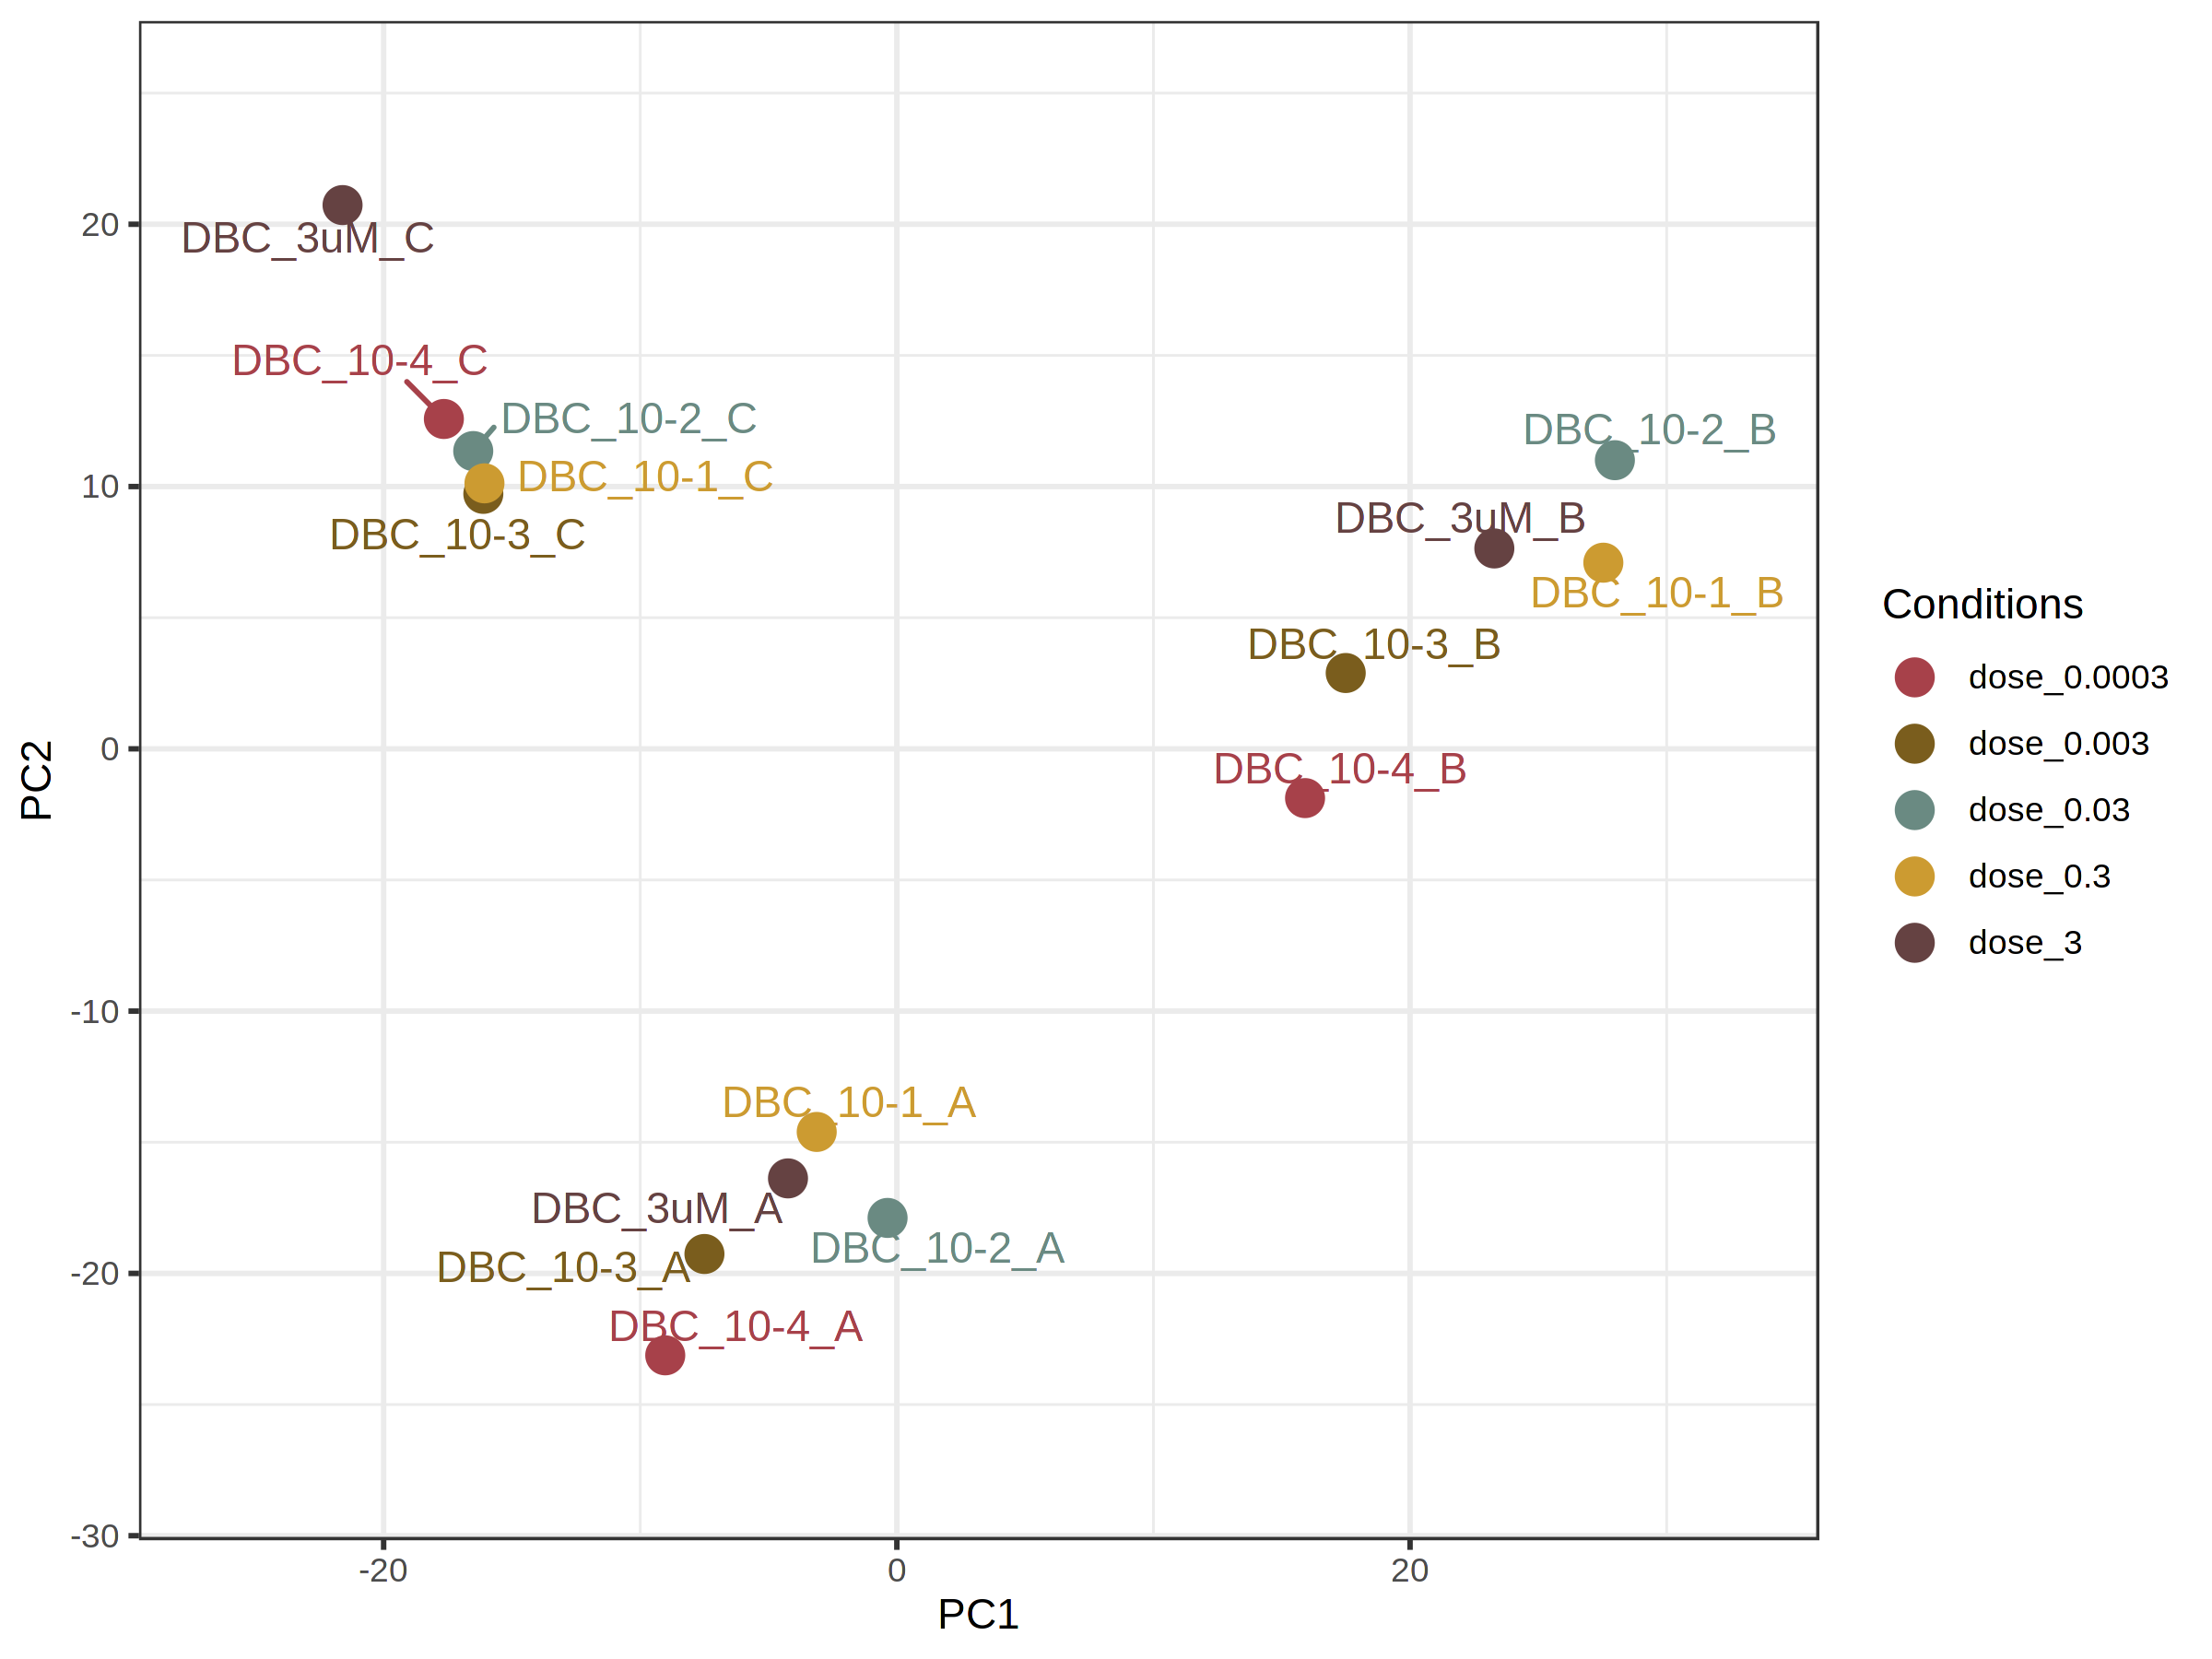
\includegraphics[width=0.8\textwidth]{qc_pca_0dpi72.png}
\caption{
PCA plot of raw uploaded data.
}
\end{center}
\label{qc_pca_0dpi72.png}
\end{figure}
\begin{figure}[htp]
\begin{center}
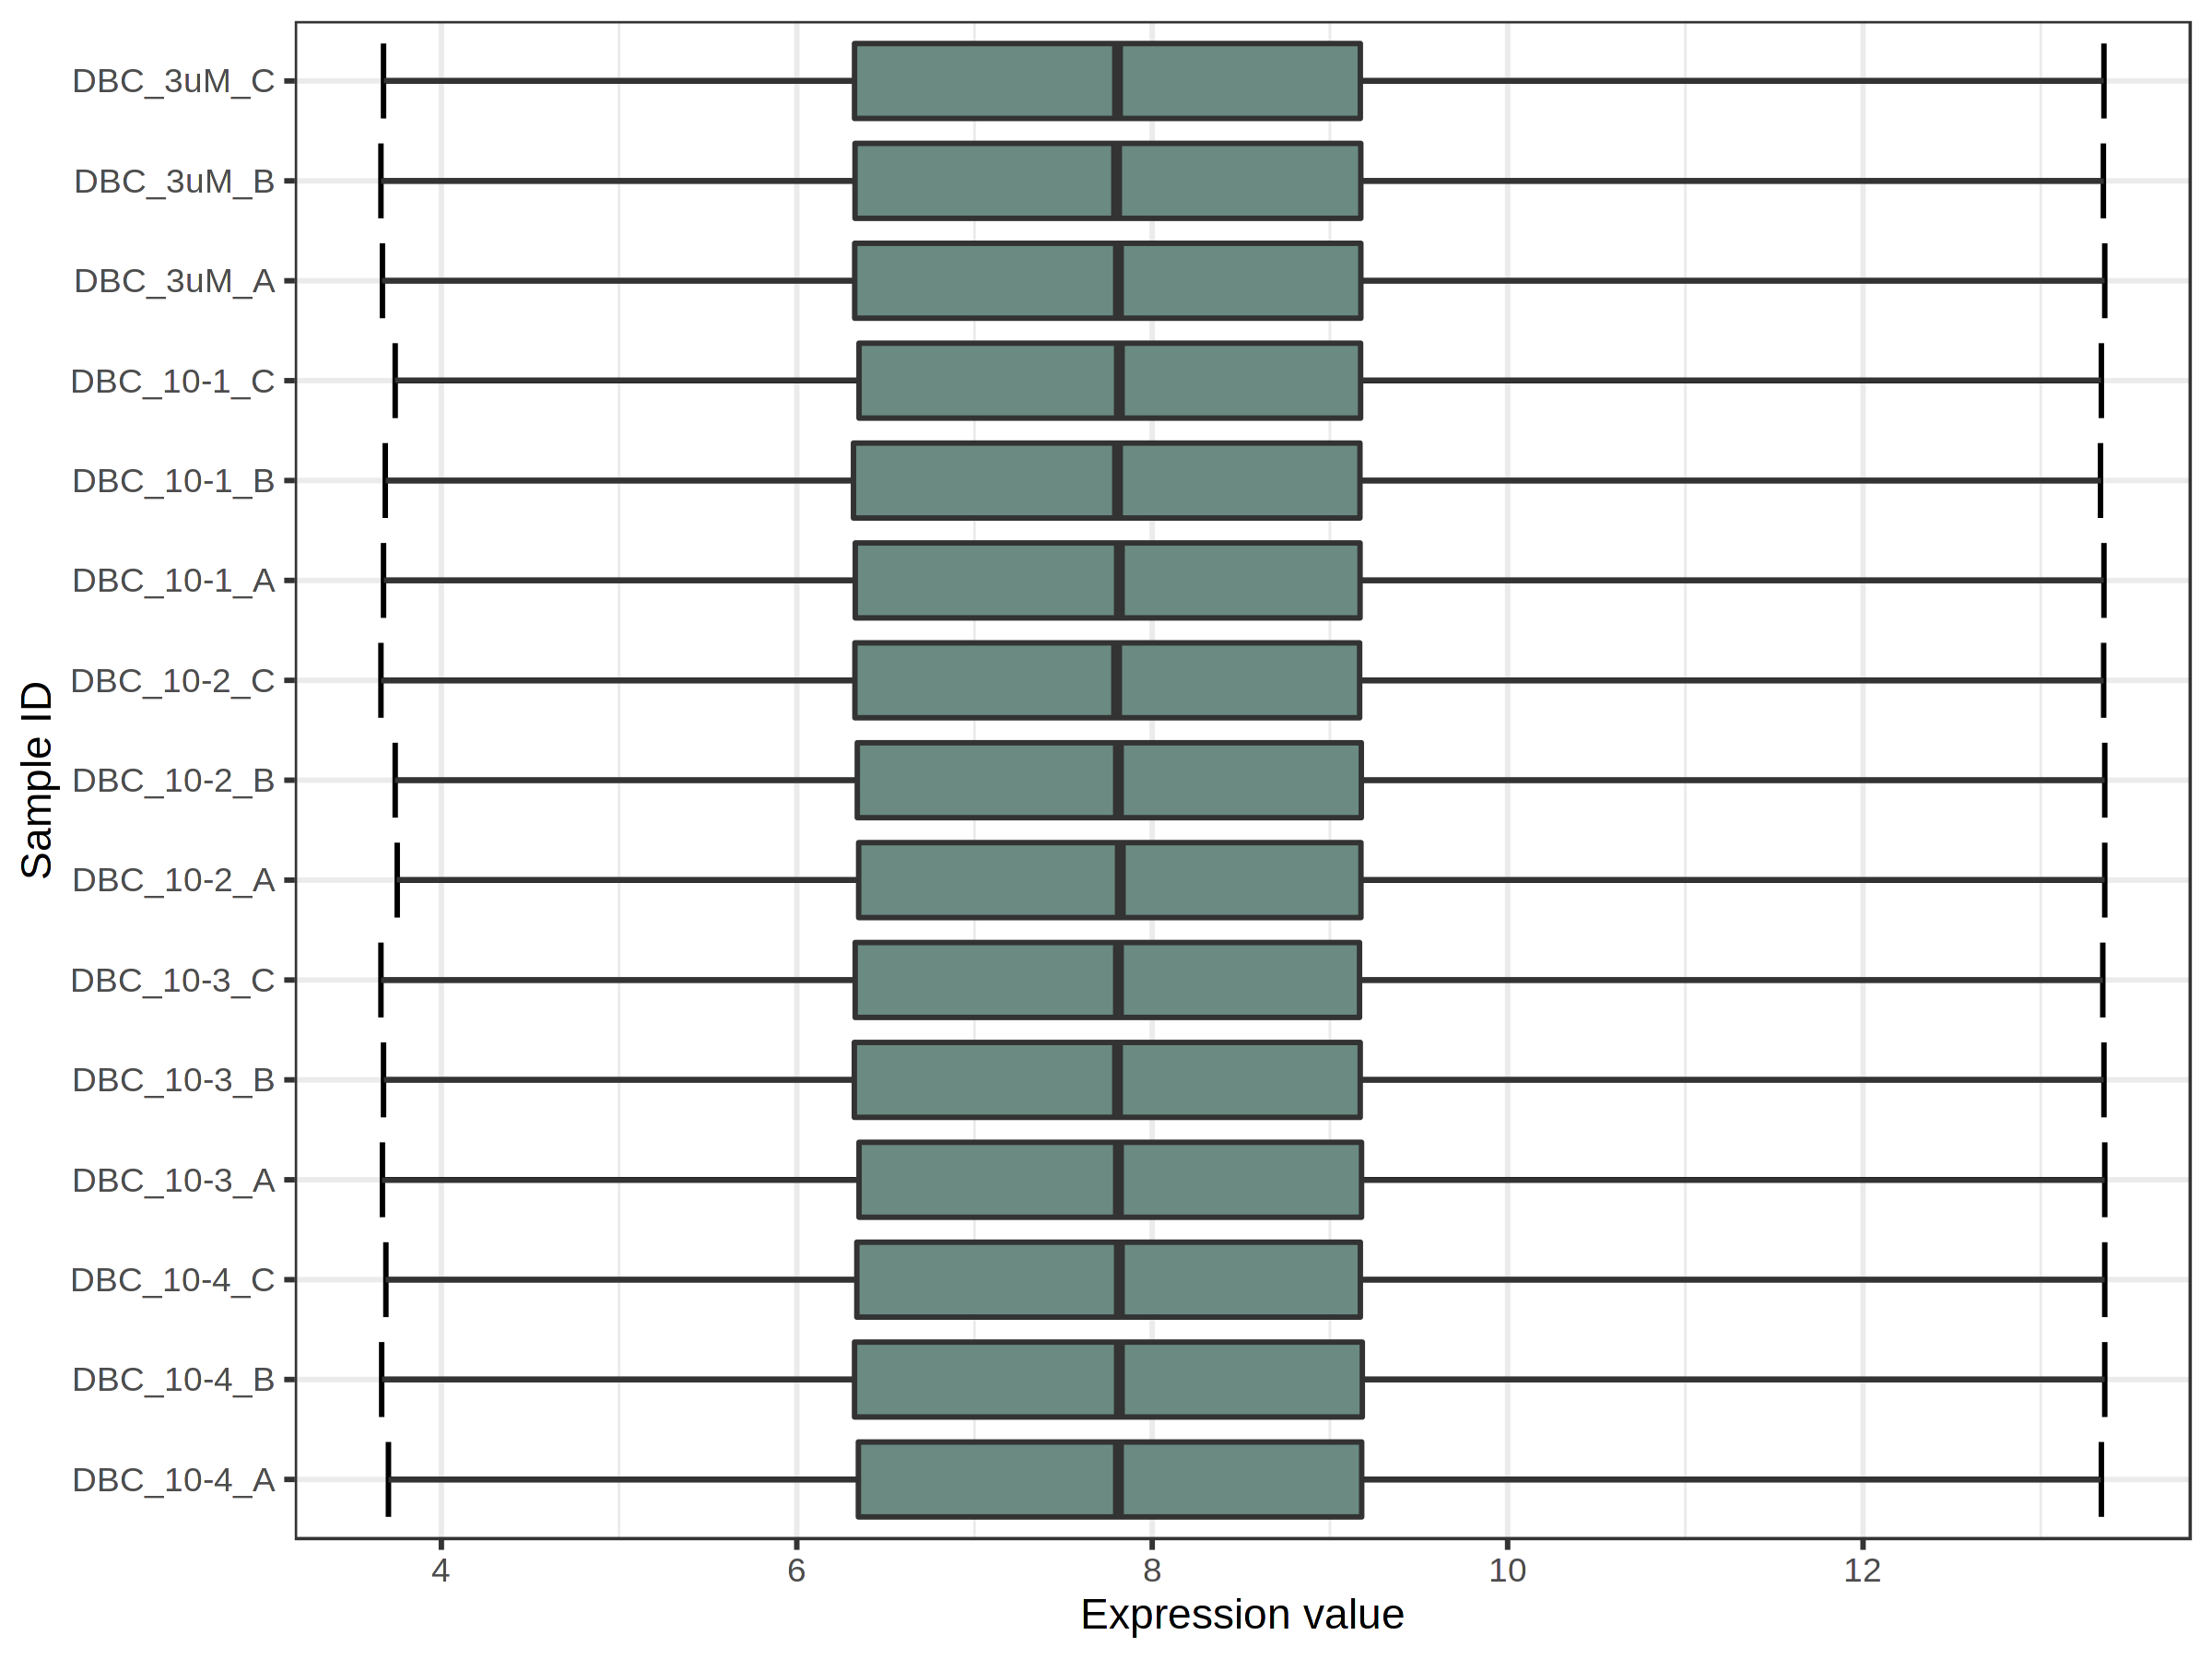
\includegraphics[width=0.8\textwidth]{qc_boxplot_0dpi72.png}
\caption{
Box plot of raw uploaded data.
}
\end{center}
\label{qc_boxplot_0dpi72.png}
\end{figure}
\section{Normalization and Filtering}
 Filtering removes data that are unlikely to be informative or are simply erroneous.  Normalization ensures that the distribution of expression values for each sample are similar across the entire experiment.  It is crucial for statistically robust and reliable detection of transcriptional differences across treatment groups.  Figures 3 and 4 summarize the data after normalization. The parameters that you chose for this section are  summarized in the bullets below:  \begin{itemize} \item{Variance filter percentile:  0 } \item{Abundance filter percentile:  0 } \item{Normalization method:  none } \end{itemize} 

\begin{figure}[htp]
\begin{center}
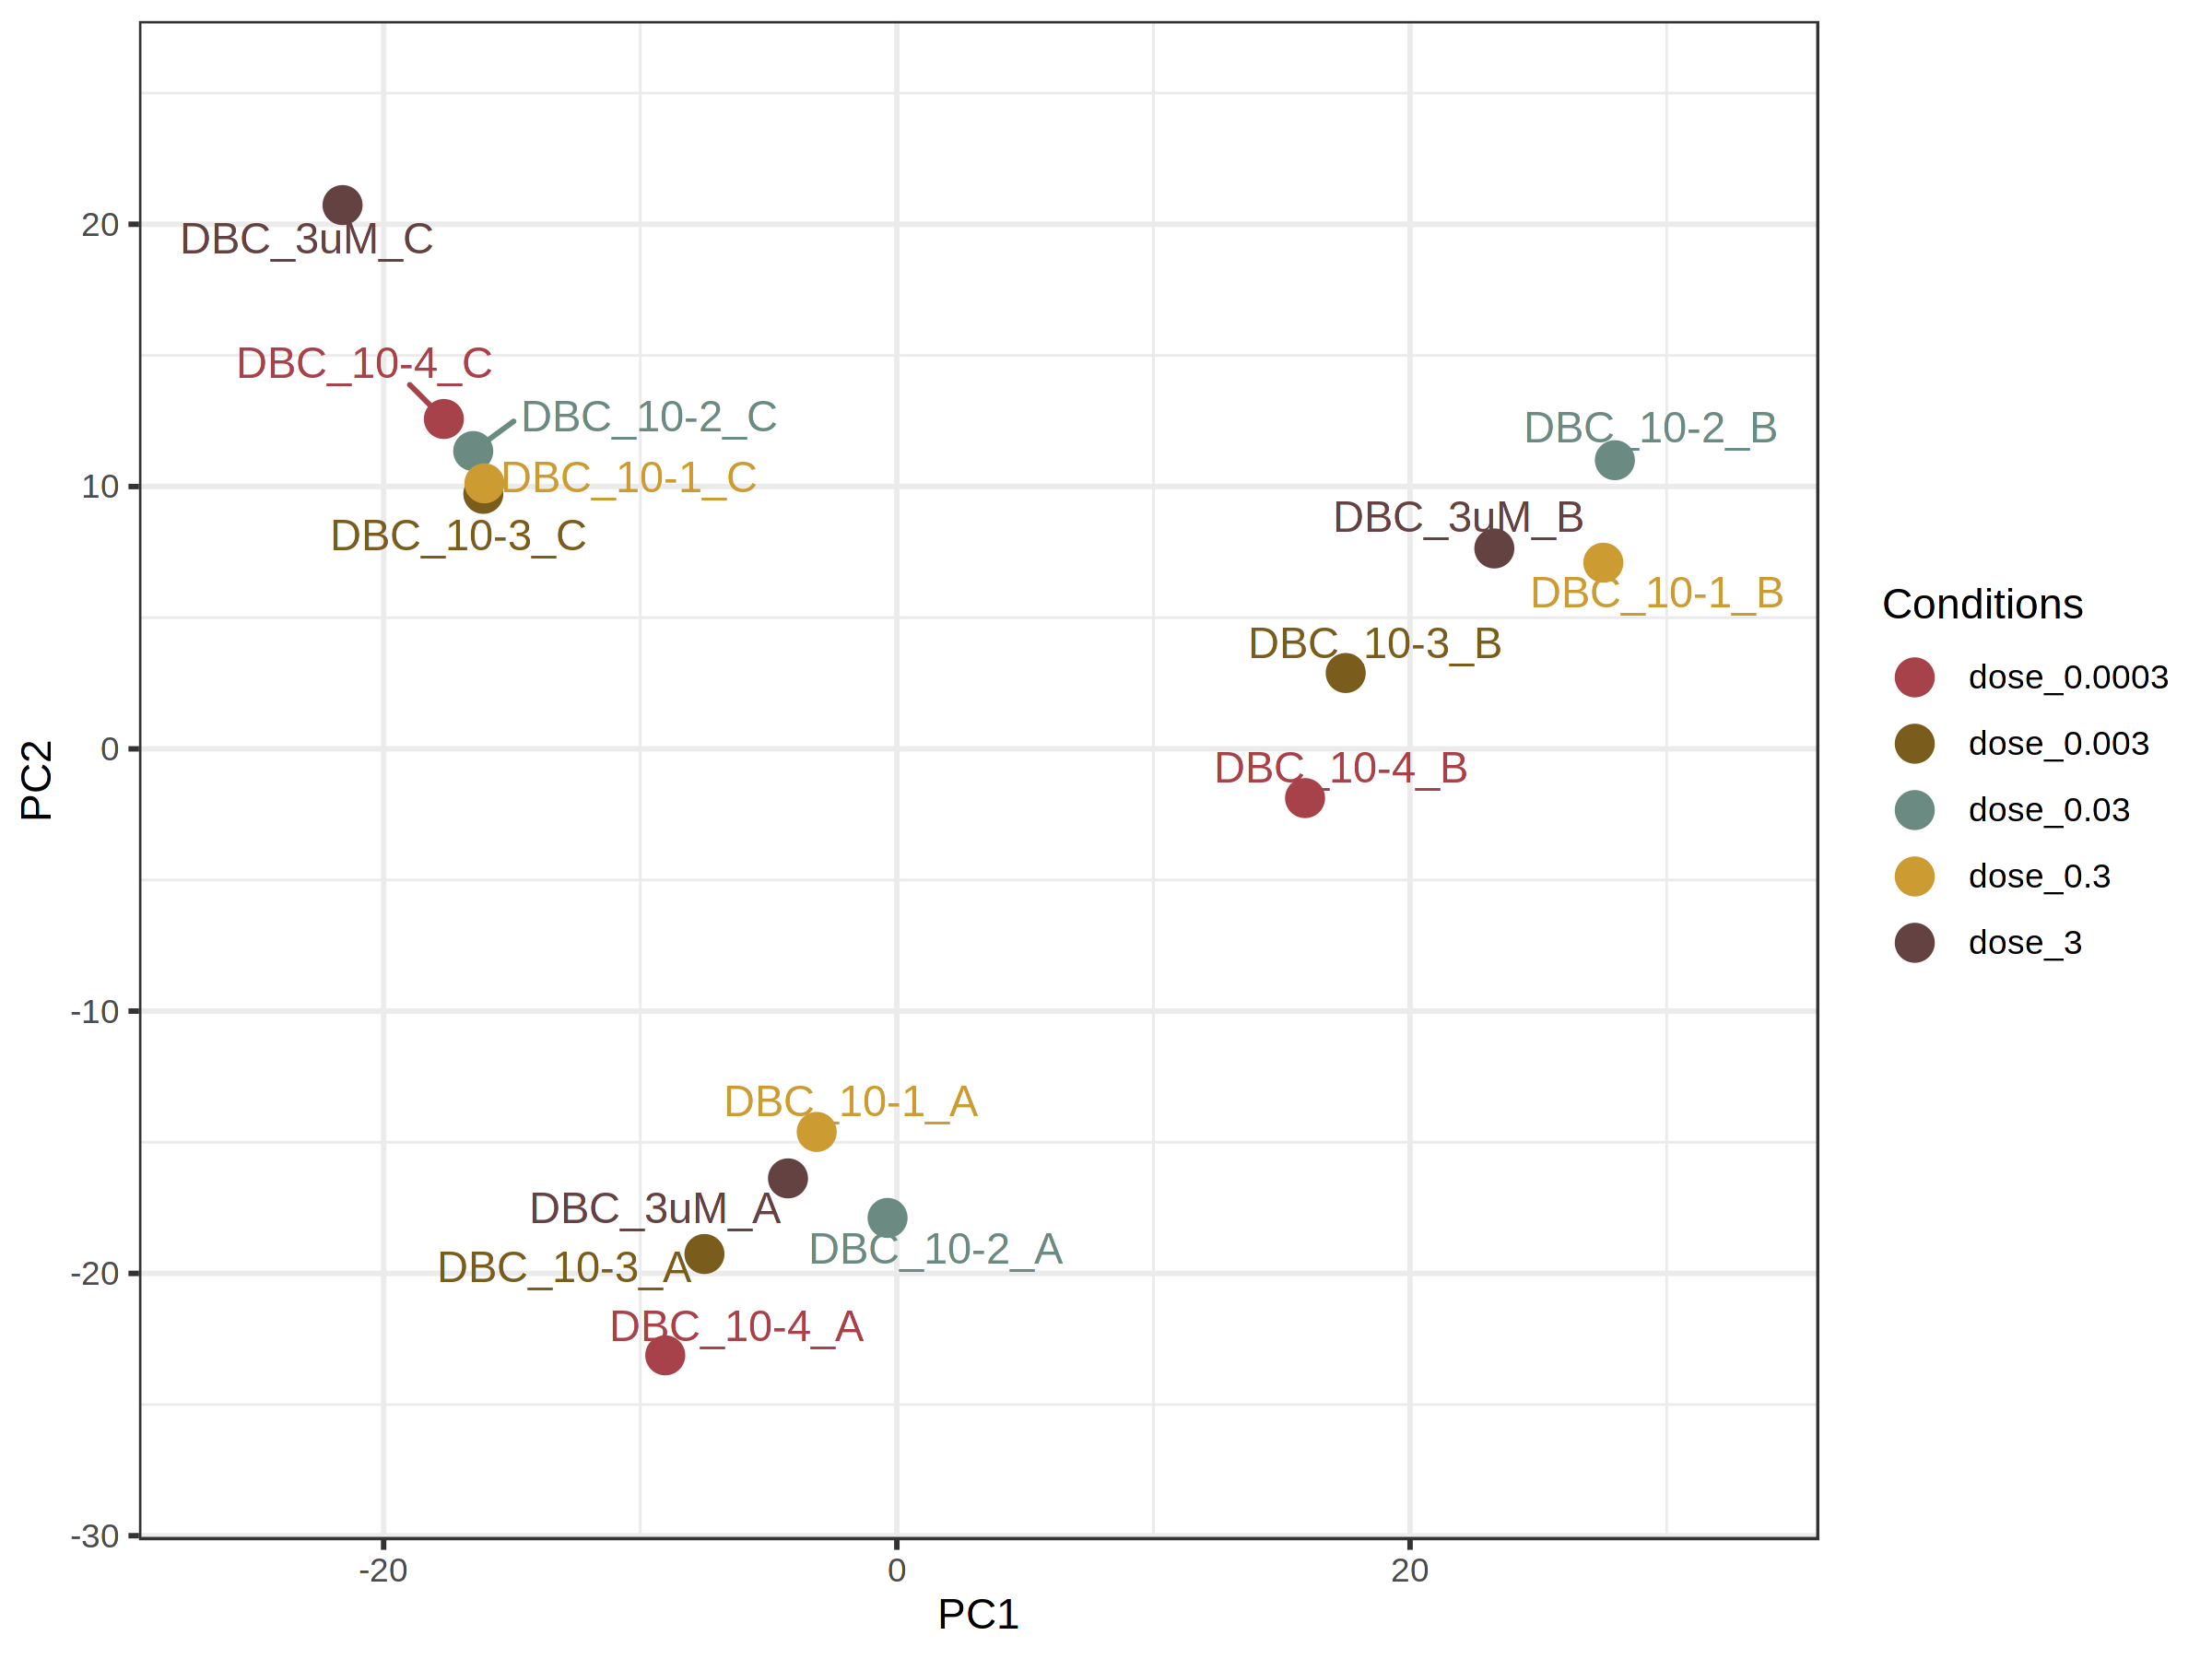
\includegraphics[width=0.8\textwidth]{qc_norm_pca_0dpi72.png}
\caption{
PCA plot of normalized data.
}
\end{center}
\label{qc_norm_pca_0dpi72.png}
\end{figure}
\begin{figure}[htp]
\begin{center}
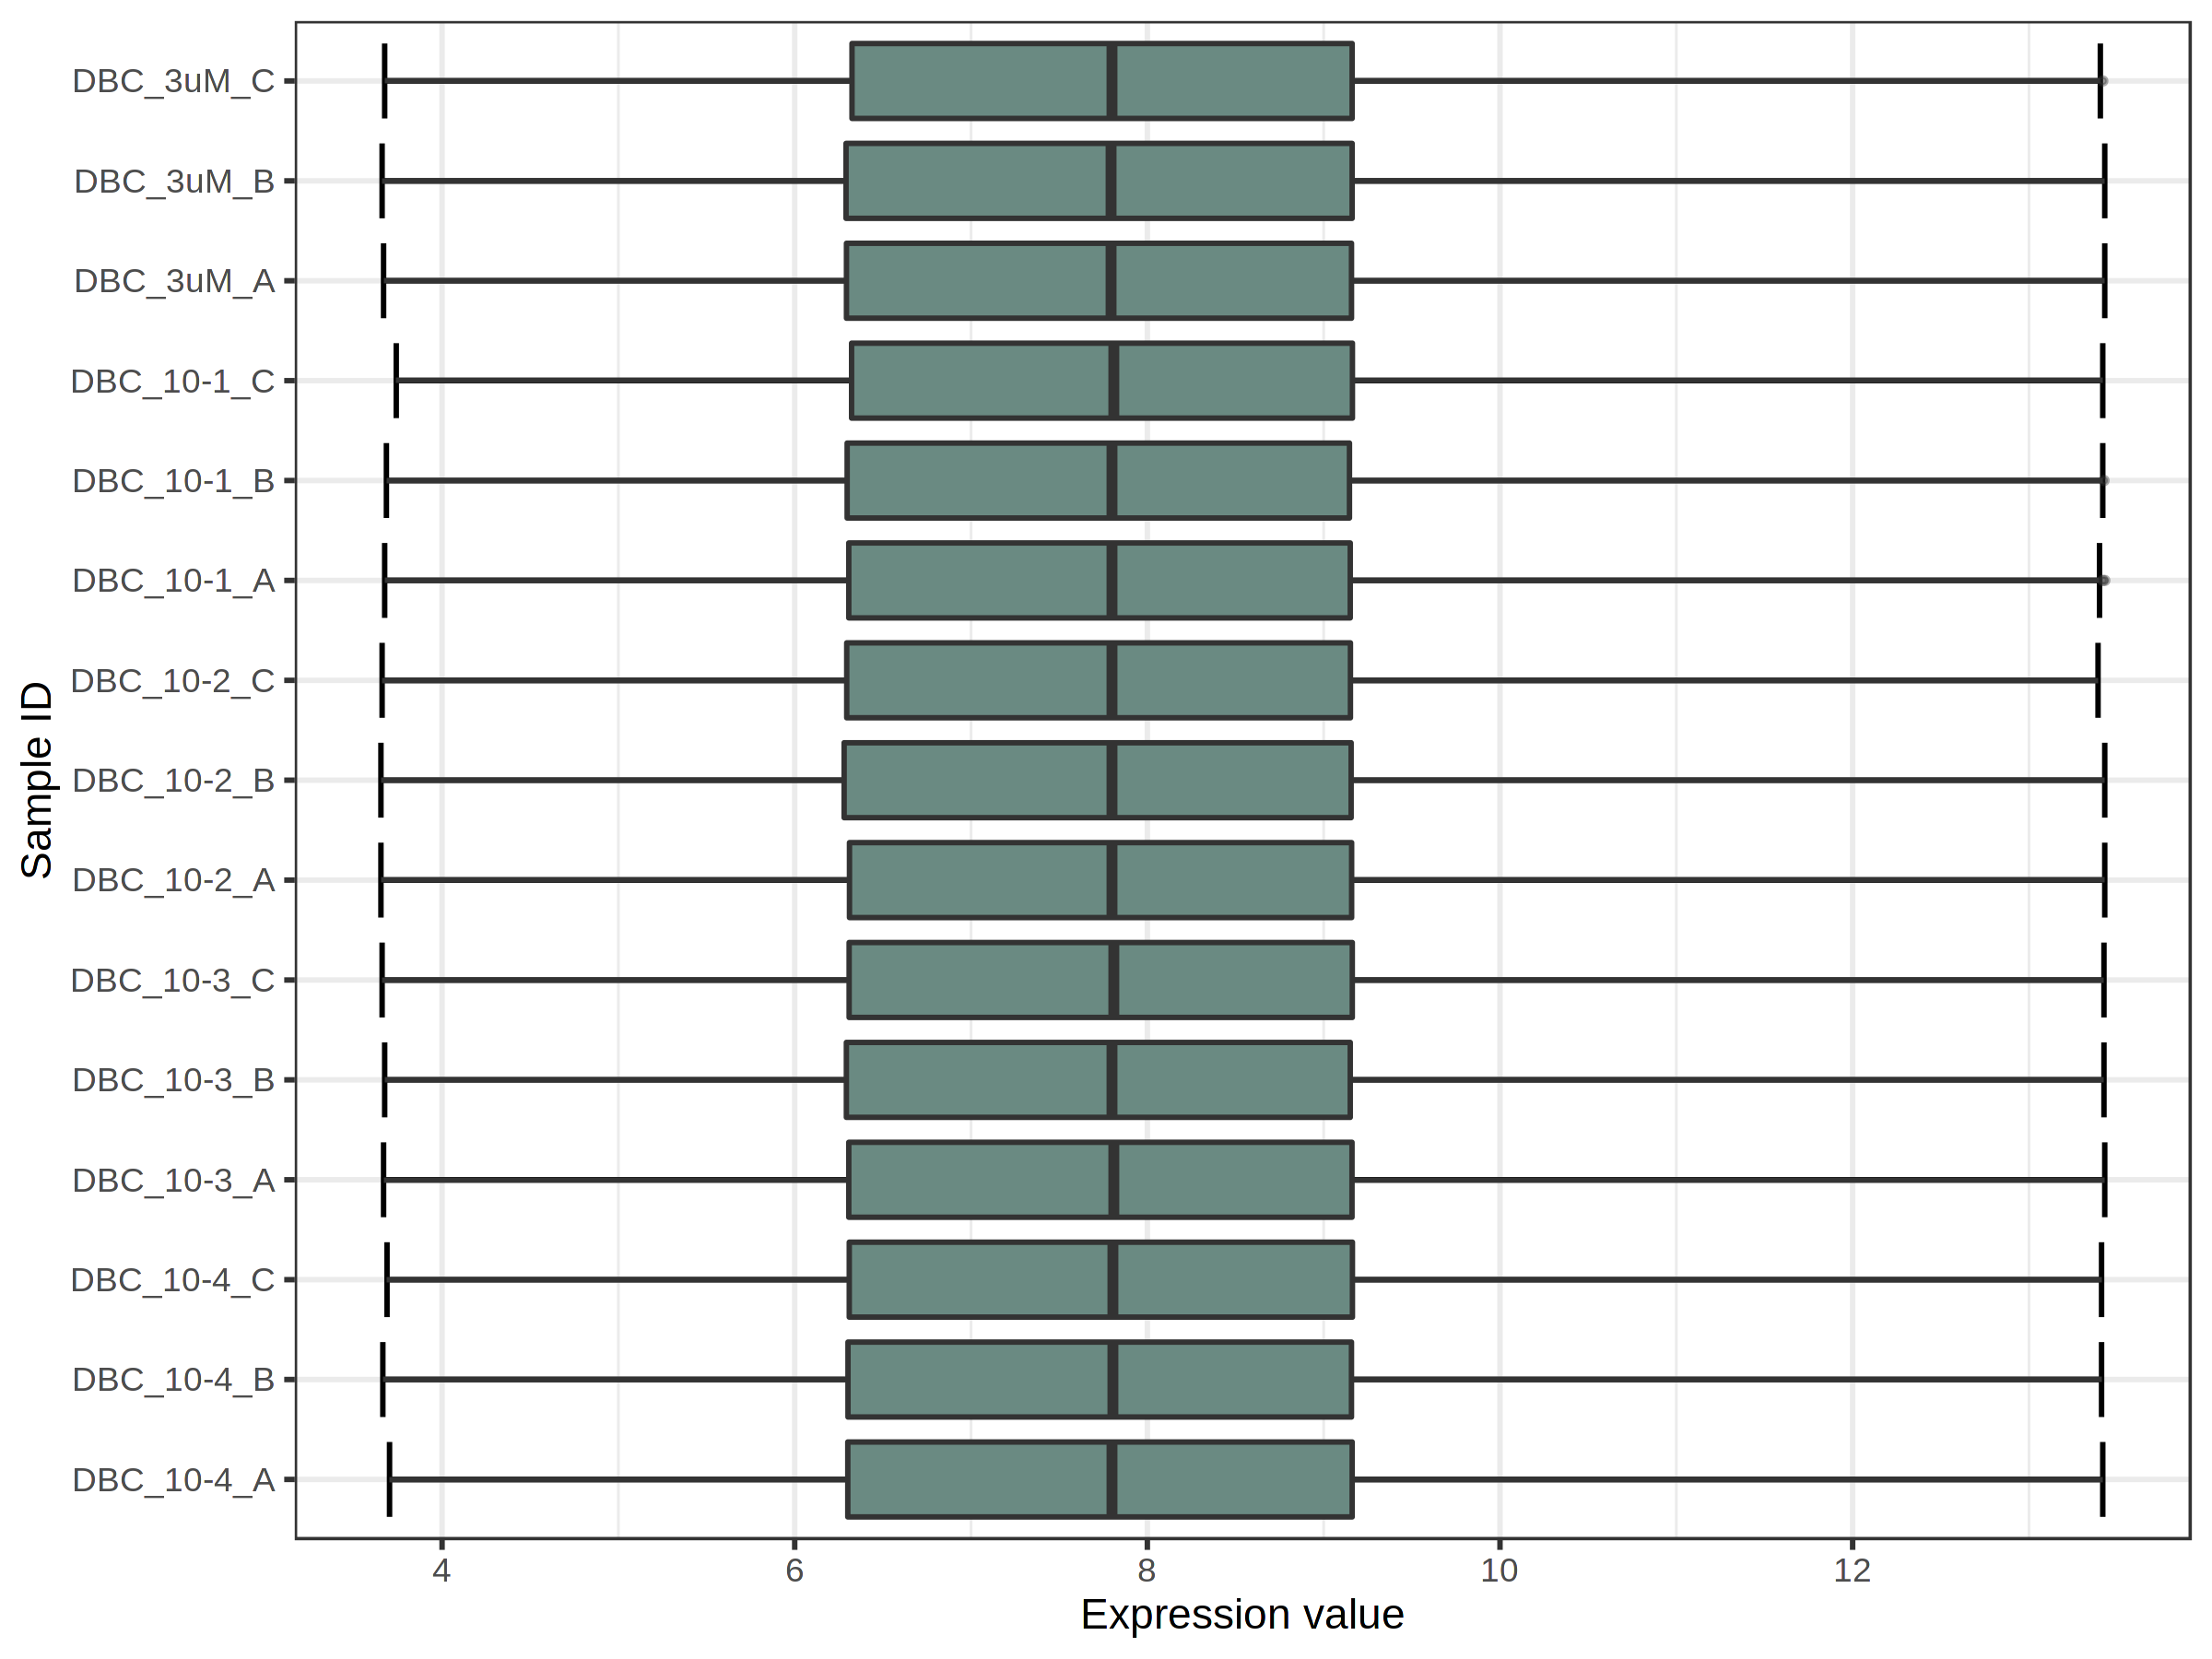
\includegraphics[width=0.8\textwidth]{qc_norm_boxplot_0dpi72.png}
\caption{
Box plot of normalized data.
}
\end{center}
\label{qc_norm_boxplot_0dpi72.png}
\end{figure}
\section{Differential Expression Analysis}
 Prior to the computationally intensive curve fitting steps, genes are removed that are unlikely to have a dose-dependent behavior  based on fold-changes and p-values computed using Limma. Since genes will be subject to additional filters during the curve-fitting  steps, it is convention to use relaxed thresholds compared to traditional differential expression analysis. However, if there is a  strong transcriptomic response, we recommend increasing the threshold values such that less than 800 genes pass this step for best  performance of the interactive pathway-level BMD analysis. The parameters that you chose for this section are listed below:  \begin{itemize} \item{Control condition: $ dose_0.0003 $} \item{P-value:  0.05 } \item{FDR:  false } \item{log2FC:  1 } \end{itemize} 

\section{Curve Fitting and Gene-level BMDs}
 To calculate gene-level BMDs, up to 10 statistical models are fit to the expression of each gene. Any model  fits with a poor fit are filtered out, and then the best fitting model is chosen based on AIC. The selected fit is  used to compute the BMD. We recommend selecting all statistical models except for Poly3 and Poly4, which should only  be used if you expect a non-monotonic response. These higher order polynomials should be used with caution since they  sometimes have unpredictable behavior, especially for dose-response experiments with a log-scale dosing scheme.  Figure 5 is a density plot showing the distribution of geneBMDs with vertical lines for the omicBMDs. Figure 6  is a bar plot showing the breakdown of best fit models. The parameters that you chose for this section are listed below:  \begin{itemize} \item{Selected statistical models:  Exp2 Exp3 Exp4 Exp5 Poly2 Lin Power Hill } \item{Lack-of-fit p-value:  0.1 } \item{BMR factor:  1 } \end{itemize} 

\begin{figure}[htp]
\begin{center}
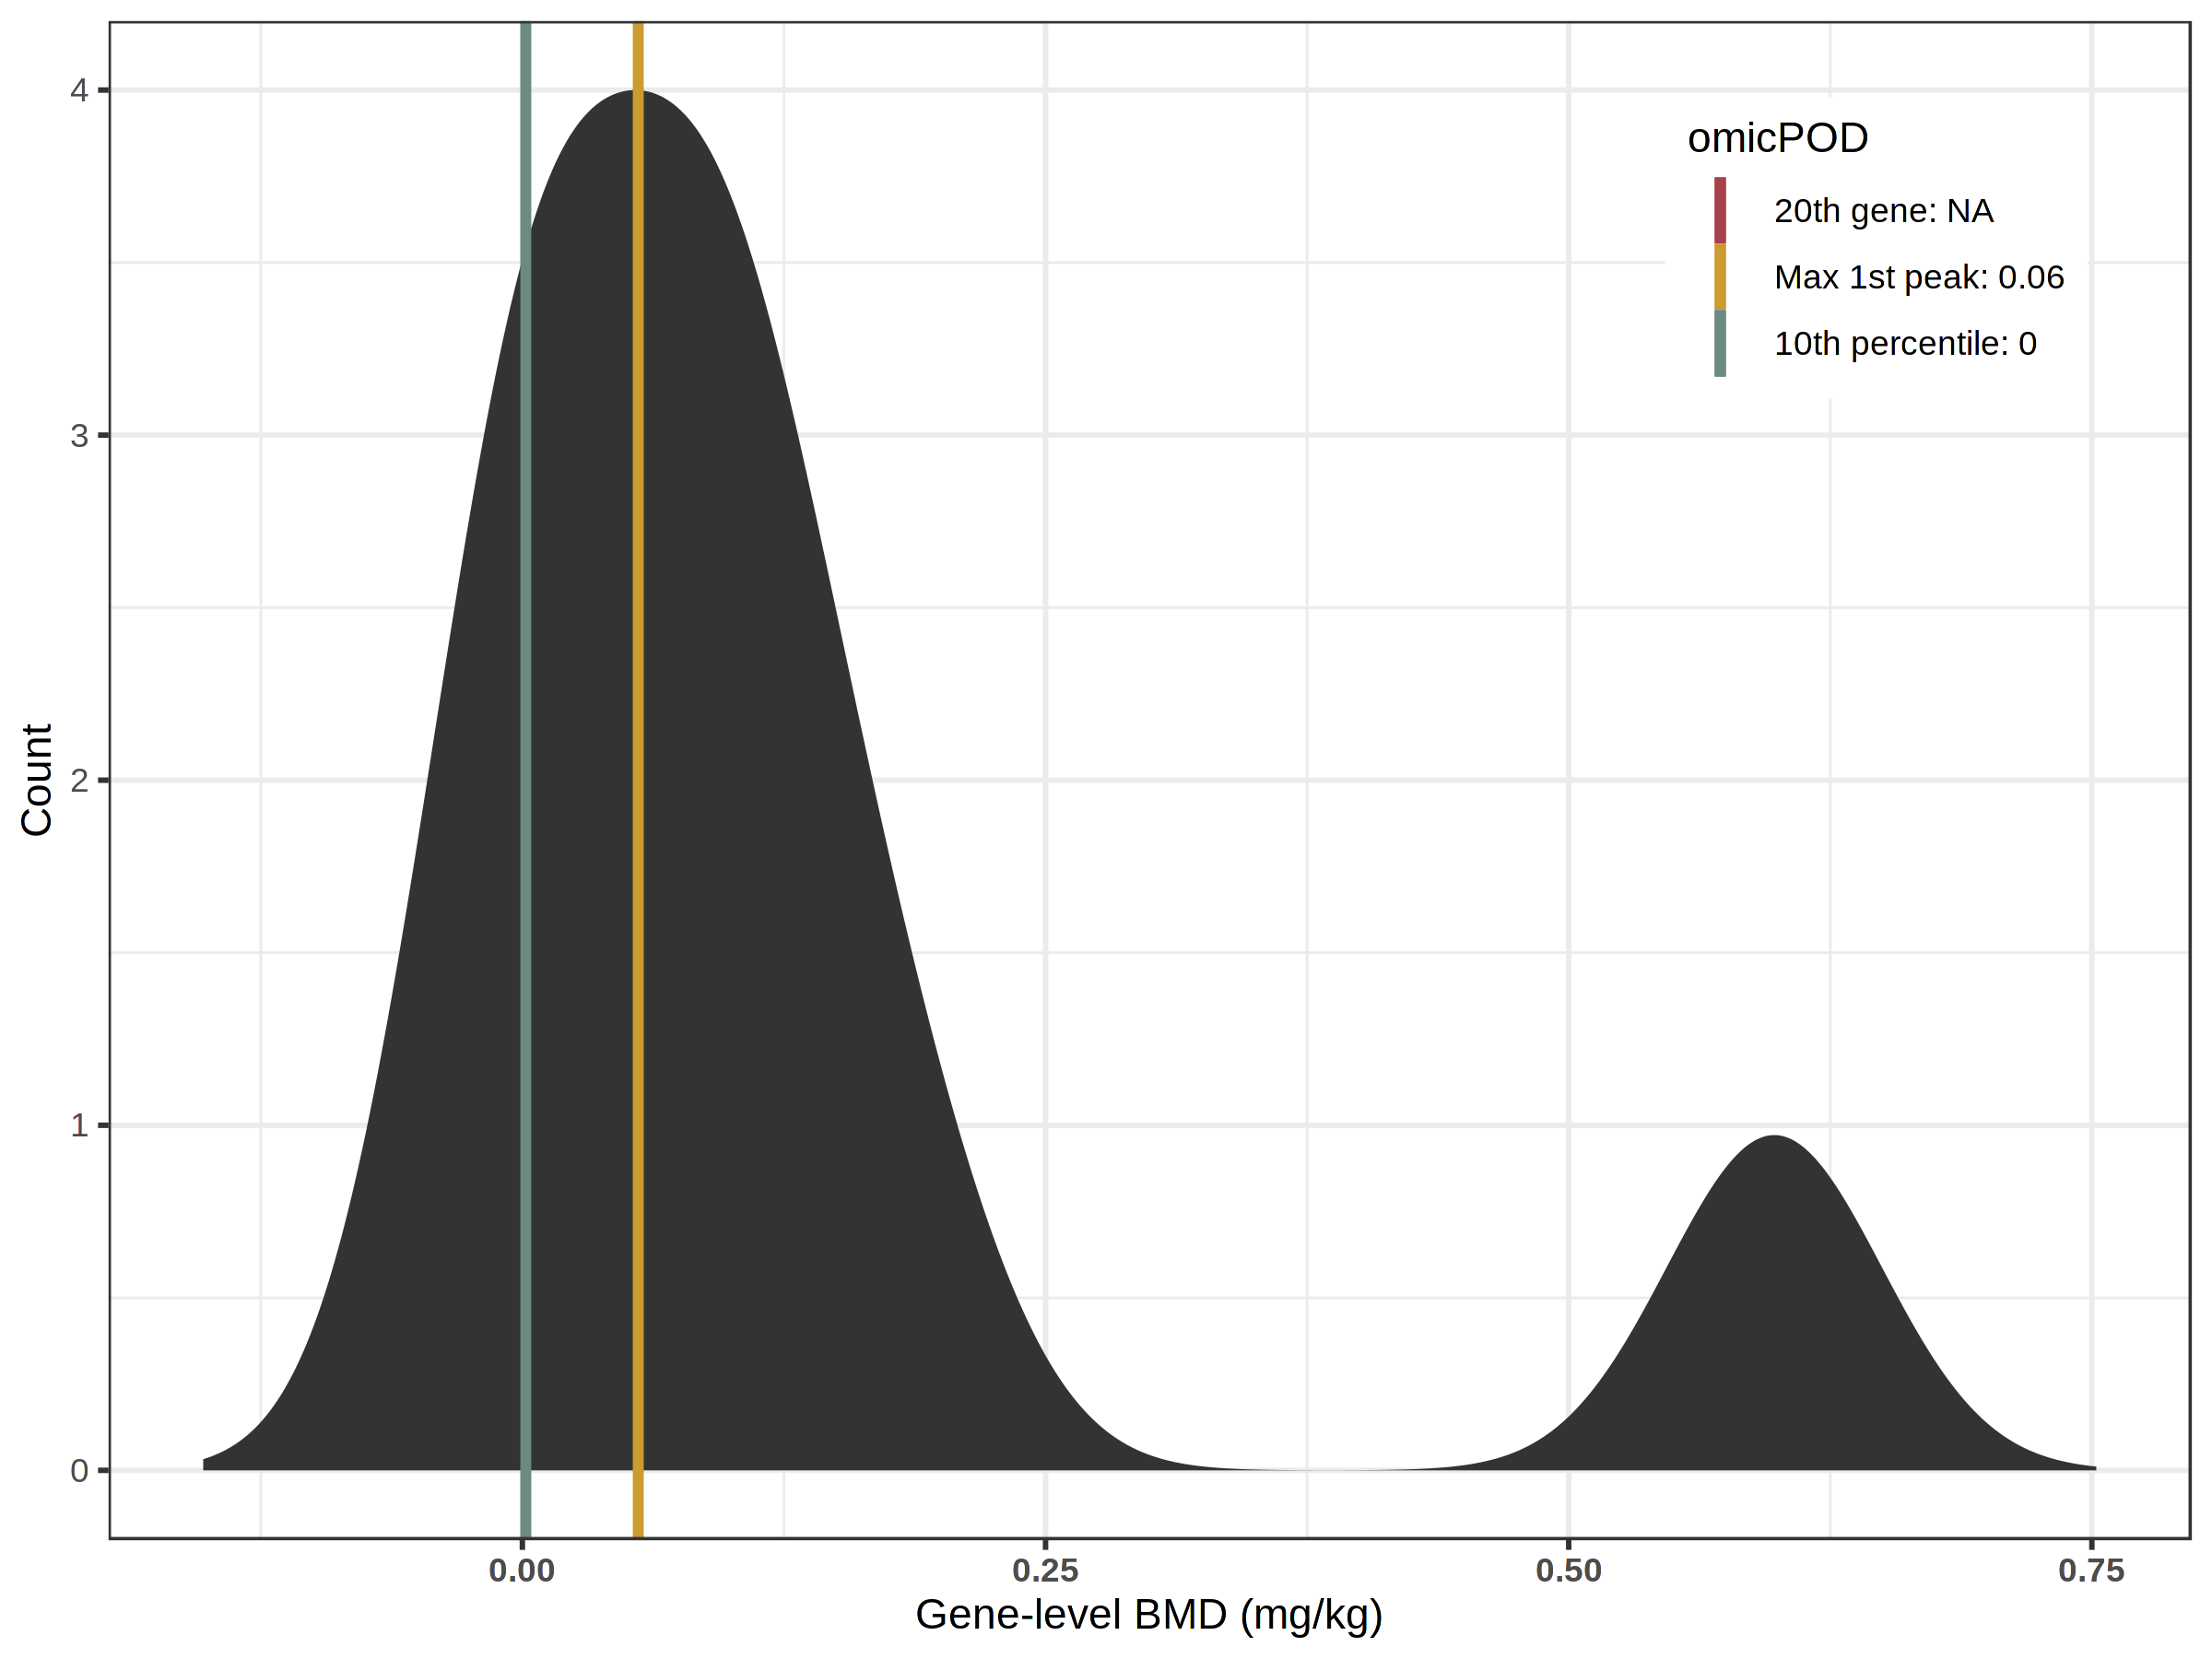
\includegraphics[width=0.8\textwidth]{dr_histogram_0dpi72.png}
\caption{
Density plot of gene-level benchmark doses (BMDs).
}
\end{center}
\label{dr_histogram_0dpi72.png}
\end{figure}
\begin{figure}[htp]
\begin{center}
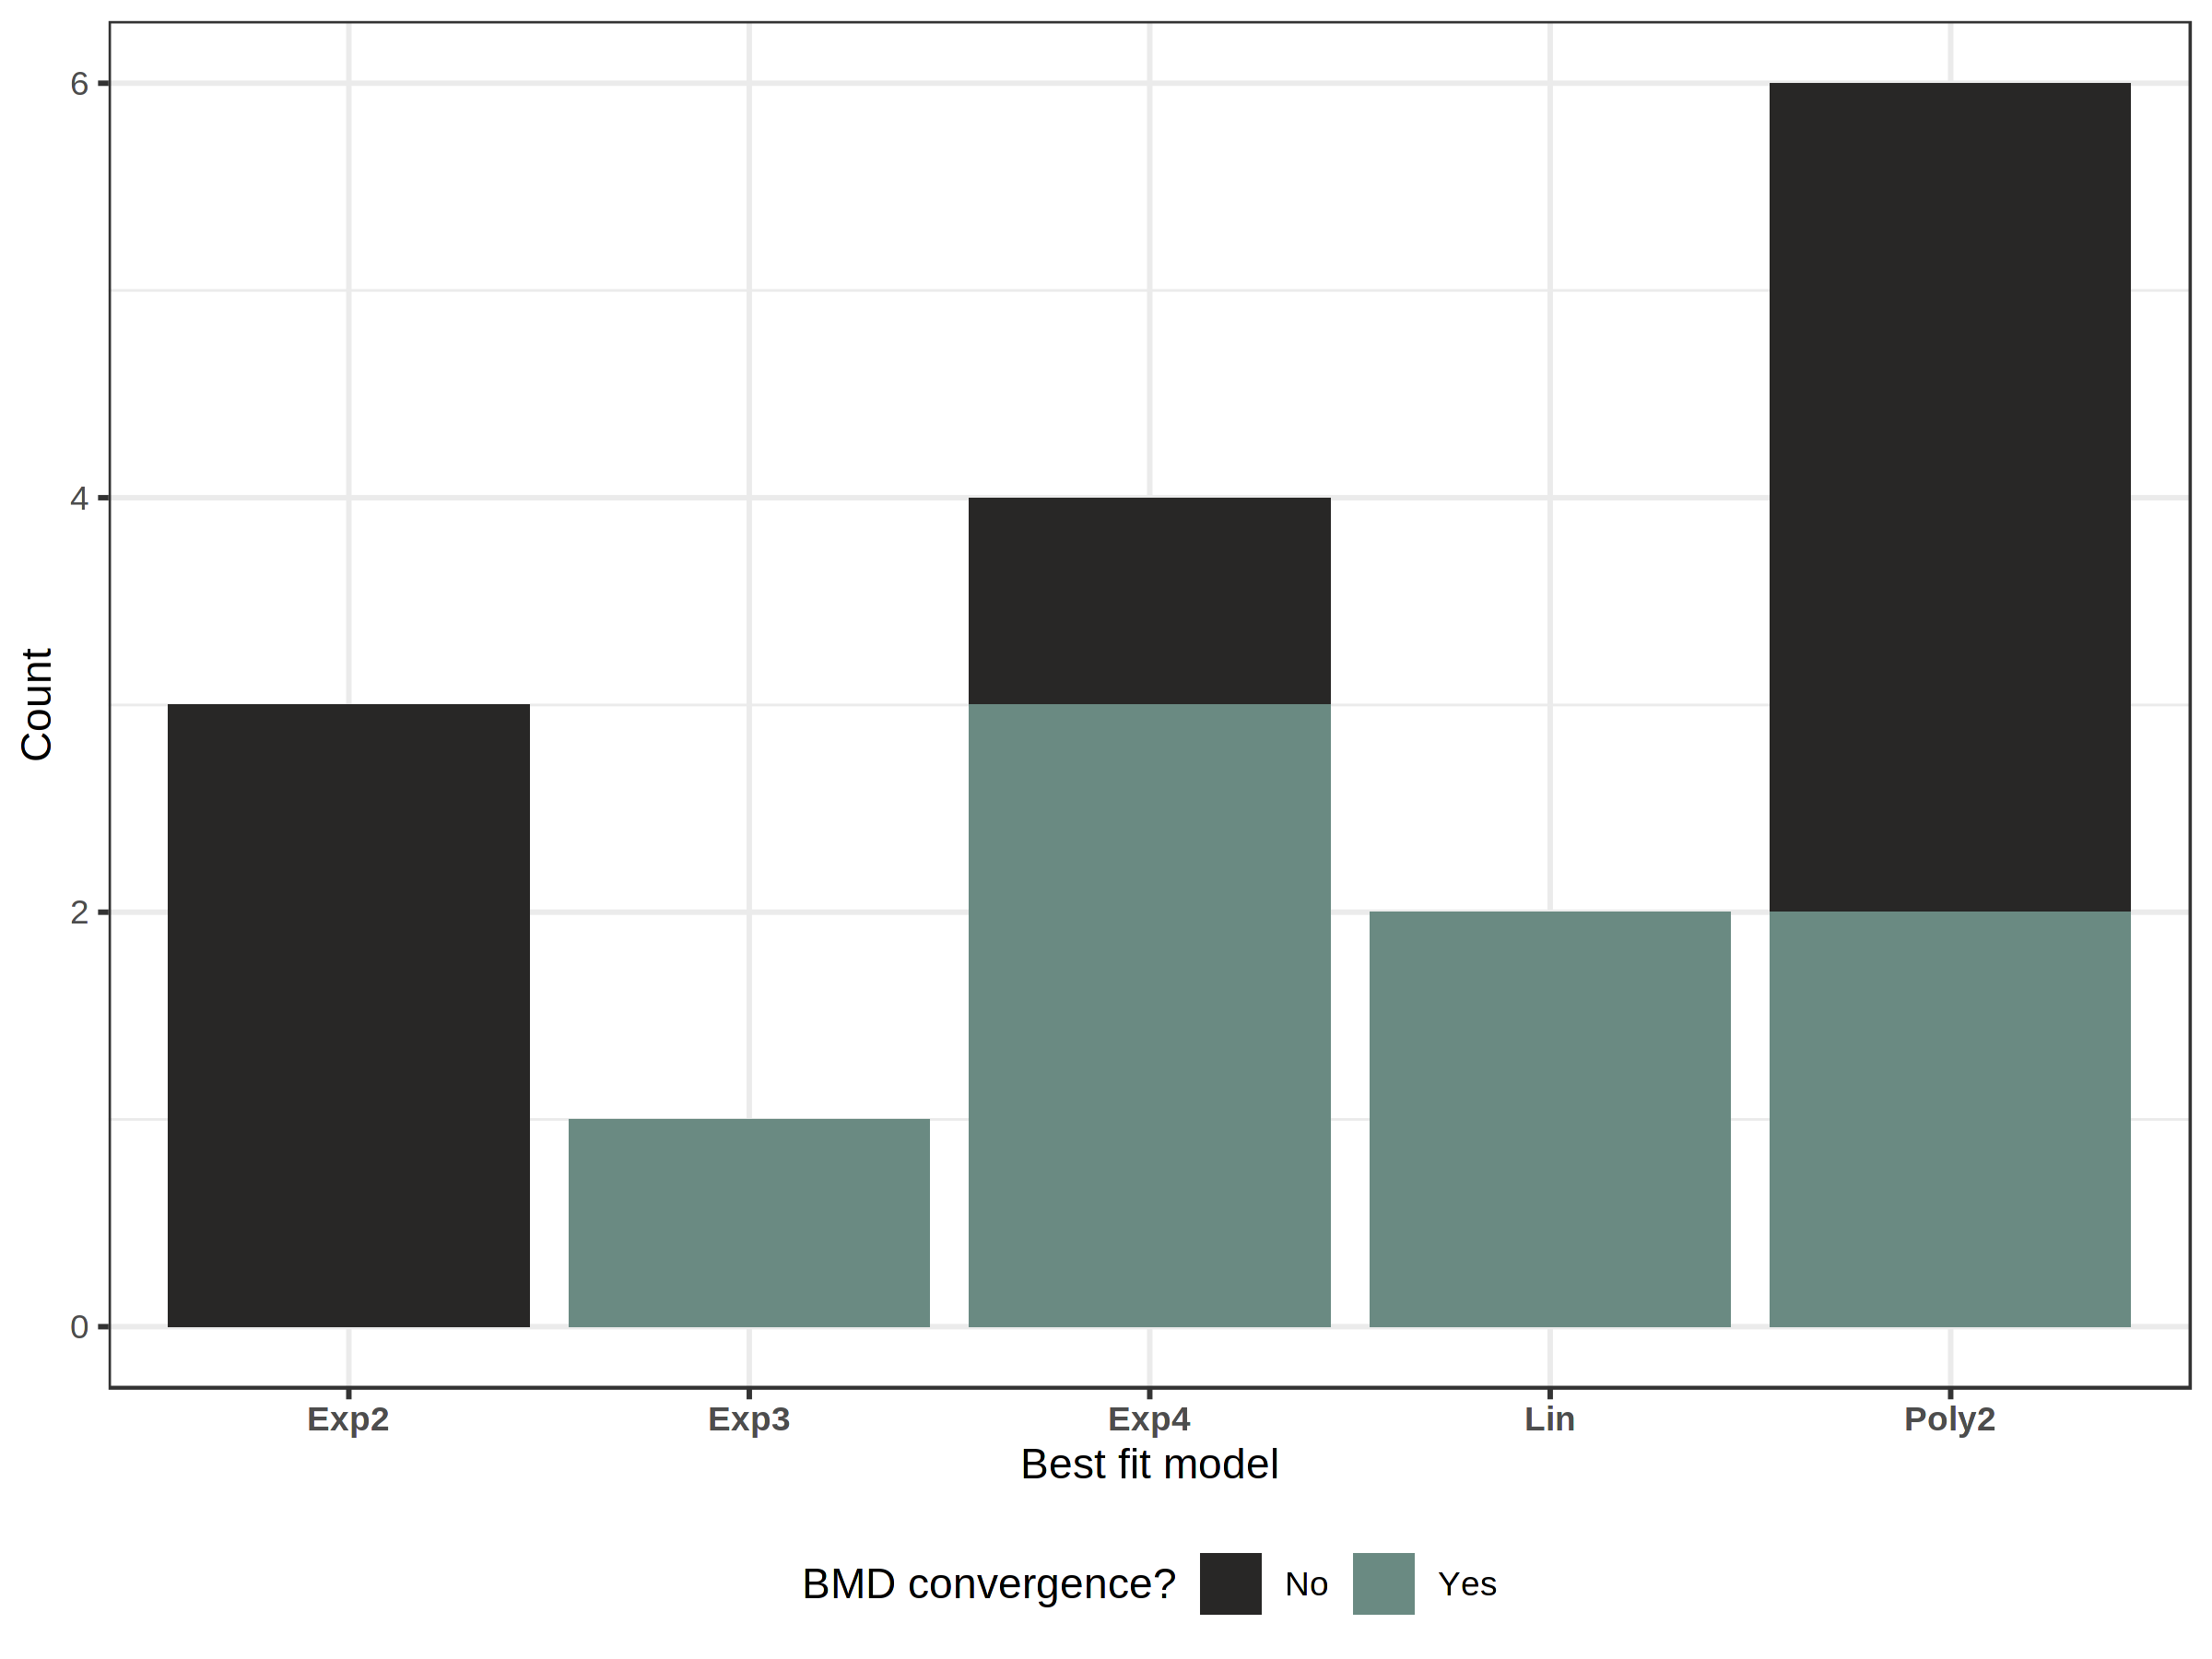
\includegraphics[width=0.8\textwidth]{dr_barplot_0dpi72.png}
\caption{
Frequency of statistical models among best fit curves.
}
\end{center}
\label{dr_barplot_0dpi72.png}
\end{figure}
\vspace{5 mm}
--------------------------------

 The report was generated on Fri Apr 24 14:23:53 2020 with R version 3.6.3 (2020-02-29).
 \end{document}

